\documentclass{article}

\usepackage[submission]{colm2026_conference}

\usepackage{microtype}
\usepackage{hyperref}
\usepackage{url}
\usepackage{booktabs}
\usepackage{graphicx}
\usepackage{lineno}

\definecolor{darkblue}{rgb}{0, 0, 0.5}
\hypersetup{colorlinks=true, citecolor=darkblue, linkcolor=darkblue, urlcolor=darkblue}

\title{When Self-Consistency Backfires: Majority Vote Hurts the Majority of Expert-Level Problems}

% Authors must not appear in the submitted version.
% The submission option handles this automatically, but verify before uploading.
\author{Anonymous}

\newcommand{\fix}{\marginpar{FIX}}
\newcommand{\new}{\marginpar{NEW}}

\begin{document}

\ifcolmsubmission
\linenumbers
\fi

\maketitle

\begin{abstract}
Self-consistency (SC) via majority vote is a widely used way to spend
inference-time compute: sample $N$ chains of thought, return the plurality
answer. On the full GPQA Diamond benchmark (198 graduate-level science
questions), majority voting reduces per-problem accuracy on a majority of
problems for two instruction-tuned models from different families: 56.6\% of
problems for Qwen2.5-7B and 65.7\% for Llama-3-8B. The effect was
pre-registered on a 151-problem confirmatory split after being observed on
47 exploratory problems, and all four confirmatory hypotheses passed. A grid
oracle that routes each problem to the best $N$ across $\{1,2,4,8,16,32,64\}$
marks a theoretical upper bound 14 accuracy points above $N=1$ for Qwen and
17 for Llama, but no verifier-free gate approaches it: a plurality-agreement
gate captures 19\% and 23\% of that headroom respectively, and a
token-entropy gate captures under 1\%, each leaving accuracy statistically
indistinguishable from fixed-budget voting. The mechanism is direct:
confidence does not track correctness on these problems. In the
highest-agreement bin the plurality answer is correct about half the time for
Qwen, and for Llama accuracy actually decreases with agreement. We
pre-register and confirm these findings on small instruction-tuned models; we
do not test reasoning-native models, which we flag as the central open
question.
\end{abstract}

\section{Introduction}

Inference-time compute is a primary lever for LLM reasoning, and
self-consistency---sample several chains of thought, return the plurality
answer---is among the simplest and most widely used techniques in this
family~\citep{wang2023self}. It is commonly assumed to be a low-risk
accuracy boost: sample more, vote, do at least as well.

That assumption fails on hard problems. When a model places its highest
probability on an incorrect answer across independent samples, more samples
only entrench the wrong vote. We call this \emph{backfire}:
$\text{mv\_gain} = \text{MV\_acc}(64) - \text{MV\_acc}(1) < 0$. We then ask
the question a cost-conscious practitioner would ask: can a cheap,
verifier-free signal computed from a few samples tell you which problems to
vote on and which to skip? We test the two most natural signals, plurality
agreement and token-level entropy, and find both fail, and we identify why.

That self-consistency can hurt is not itself new, and the underlying
miscalibration is well documented~\citep{guo2017calibration,
kadavath2022language}. Our contribution is to quantify, pre-register, and
confirm how often it happens on a full hard benchmark, across two model
families, and to show that two cheap gates cannot prevent it.

\textbf{Contributions:}
\begin{itemize}
  \item On all 198 GPQA Diamond problems, majority voting backfires on the
        majority of problems for two model families (56.6\% and 65.7\%). The
        effect was pre-registered on a 151-problem held-out split and confirmed
        (all four hypotheses passed).
  \item We show the per-problem routing headroom is real: a grid oracle (best
        $N$ per problem across $\{1,2,4,8,16,32,64\}$) marks a 14 to 17 point
        ceiling above $N=1$. A plurality-agreement gate captures 19 to 23\% of
        that headroom; a token-entropy gate captures under 1\%. Neither reaches
        the oracle nor beats fixed-budget voting meaningfully.
  \item We give the mechanism: agreement does not track correctness, and for
        the weaker model it is anti-correlated.
\end{itemize}

\section{Setup}

\textbf{Dataset and design.} We use the full GPQA Diamond
benchmark~\citep{rein2023gpqa}, 198 graduate-level multiple-choice questions
in biology, chemistry, and physics. We adopt a pre-registered confirmatory
design: 47 problems are \textbf{exploratory} (the hypotheses below were
generated from them), and the remaining 151 are a \textbf{confirmatory} test
set. The hypotheses and thresholds were locked and git-tagged before any
confirmatory analysis. We report exploratory, confirmatory, and pooled (198)
values throughout, but decide PASS/FAIL on the confirmatory set only.

\textbf{Models.} Two instruction-tuned models from different families, served
on Together AI: Qwen2.5-7B-Instruct-Turbo and Meta-Llama-3-8B-Instruct-Lite.
Both are small (7 to 8B) and non-reasoning. $N=64$ samples per problem,
temperature 0.7, single locked prompt template (SHA-256 verified). Five-pass
answer extraction; parse rate 99.5\% (Qwen) and 98.6\% (Llama).

\textbf{Metrics.} $\text{MV\_acc}(N)$ is expected majority-vote accuracy over
$N$ samples, ties broken uniformly at random independent of ground truth,
estimated by Monte Carlo over subsets. Backfire is $\text{mv\_gain} < 0$.

\textbf{Routing and gates.} The \textbf{oracle} routes each problem to the
$N$ that maximizes majority-vote accuracy across $\{1,2,4,8,16,32,64\}$ using
ground truth; it is a theoretical upper bound, not a deployable method. The
\textbf{agreement gate} returns the probe plurality when its fraction over $k$
samples is at least $\tau$, else votes at $N=64$. The \textbf{entropy gate}
routes by a threshold on mean per-token entropy. Both gates are verifier-free;
ground truth is used only to score the result. Logprobs are available for all
151 confirmatory problems but not for the 47 older exploratory ones, so the
entropy gate is evaluated on the confirmatory set. The entropy gate threshold
is selected to maximize accuracy on the confirmatory set (Qwen: 0.113, Llama:
0.139).

\textbf{Uncertainty.} 95\% confidence intervals are problem-level bootstrap
(1000 iterations, seed 42).

\section{Pre-Registered Confirmatory Results}

All four pre-registered hypotheses pass on the 151 confirmatory problems
(Table~\ref{tab:confirmatory}). Thresholds were fixed below the exploratory
point estimates, so each is a genuine prediction rather than a restatement.
PH2 and PH4 were pre-registered against a binary $\{N=1, N=64\}$ oracle; the
grid oracle results in Sections~\ref{sec:oracle} and~\ref{sec:gates} use a
more generous ceiling and are reported separately as post-hoc analysis.

\begin{table}[t]
\begin{center}
\begin{tabular}{llllc}
\toprule
\textbf{Hyp} & \textbf{Prediction (both models)} & \textbf{Qwen2.5-7B} & \textbf{Llama-3-8B} & \textbf{Result} \\
\midrule
PH1 & backfire rate $\geq$ 33\%          & 60.3\% [53.0, 68.2] & 65.6\% [58.3, 73.5] & PASS \\
PH2 & agree gate captures $\leq$ 10\% of oracle & 0.8\%        & $-$1.6\%            & PASS \\
PH3 & top-agree-bin accuracy $\leq$ 70\% & 51.2\% ($n$=43)     & 14.3\% ($n$=21)     & PASS \\
PH4 & entropy gate captures $\leq$ 10\% of oracle & 0.5\%      & 0.9\%               & PASS \\
\bottomrule
\end{tabular}
\end{center}
\caption{Confirmatory hypotheses ($n=151$). Thresholds locked and git-tagged before analysis.}
\label{tab:confirmatory}
\end{table}

\section{Results (Pooled, 198 Problems)}

\subsection{Backfire affects the majority of problems, precisely estimated}

Majority voting reduces per-problem accuracy on most problems for both models
(Figure~\ref{fig:backfire}): the pooled backfire rate is 56.6\% (95\% CI
[49.5, 63.6]) for Qwen and 65.7\% ([59.1, 71.7]) for Llama. Expanding from
47 to 198 problems roughly halved the interval width (53\% and 55\%
narrower), and both rates sit well above the 33\% threshold.

The aggregate and per-problem pictures diverge. Voting barely moves aggregate
accuracy (Qwen 0.342 to 0.369, Llama 0.273 to 0.313) while harming the
majority of problems individually. An average that looks flat or mildly
positive can hide widespread per-problem harm. The worst single problem loses
47 points (Qwen) or 46 (Llama); a few gain as much as 66 or 71. The
asymmetry is real but rare: large gains exist, yet most problems backfire.

\begin{figure}[t]
\begin{center}
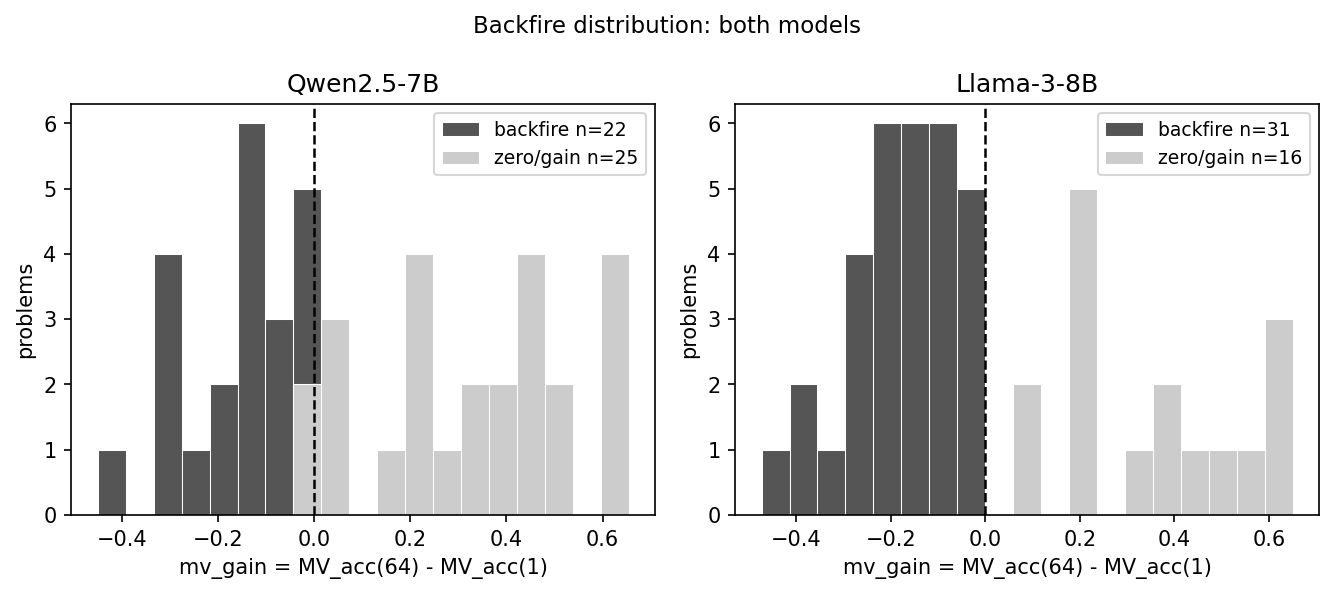
\includegraphics[width=\linewidth]{../outputs/gate_model2/backfire_both.png}
\end{center}
\caption{$\text{mv\_gain} = \text{MV\_acc}(64) - \text{MV\_acc}(1)$ per problem.
Dark bars are backfire ($\text{mv\_gain} < 0$).}
\label{fig:backfire}
\end{figure}

\subsection{The oracle upper bound is real but not reachable}
\label{sec:oracle}

A grid oracle that routes each problem to the best majority-vote accuracy
across all $N$ in $\{1,2,4,8,16,32,64\}$ reaches 0.482 (Qwen) and 0.439
(Llama), a ceiling 14 points above $N=1$ for Qwen and 17 points above for
Llama. This is a more generous bound than a binary $\{N=1, N=64\}$ oracle,
because it allows any compute level per problem. It marks how much accuracy a
perfect per-problem routing decision could recover. It is an upper bound, not
a method (Figure~\ref{fig:pareto}).

\begin{figure}[t]
\begin{center}
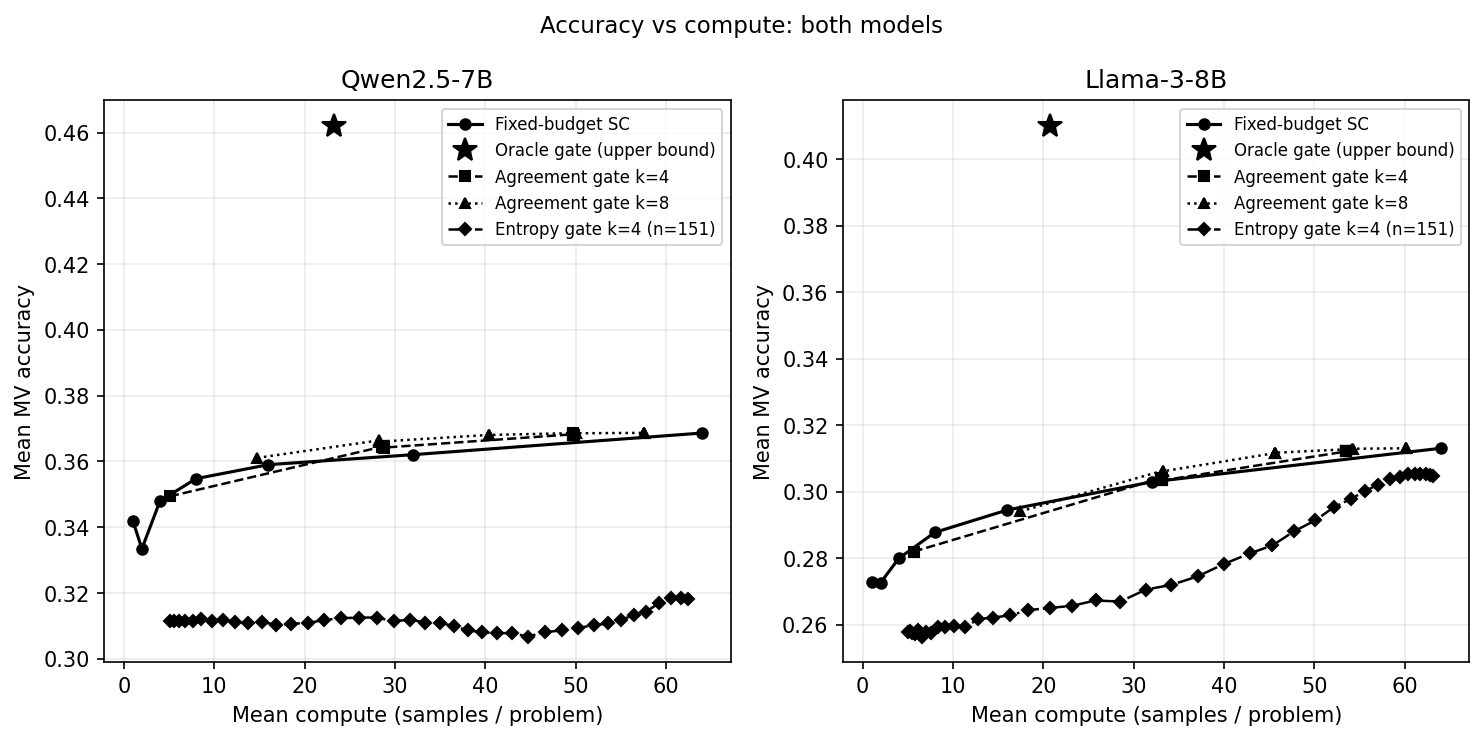
\includegraphics[width=\linewidth]{../outputs/gate_model2/pareto_both.png}
\end{center}
\caption{Accuracy vs mean compute: fixed-budget voting, the oracle upper
bound, and the verifier-free agreement and entropy gates.}
\label{fig:pareto}
\end{figure}

\subsection{Two verifier-free gates fail to capture it}
\label{sec:gates}

Neither cheap gate recovers the headroom. The agreement gate ($k=8$,
$\tau=0.75$) reaches 0.368 accuracy for Qwen and 0.312 for Llama,
statistically indistinguishable from fixed-budget voting at $N=64$ (0.369 and
0.313). Against the grid oracle ceiling, the agreement gate captures 18.7\%
of available headroom for Qwen and 23.4\% for Llama: non-trivial fractions of
a generous ceiling, yet accuracy remains flat. The entropy gate does worse: it
captures $-$16.8\% for Qwen (threshold selected on confirmatory 151 fails to
generalize to exploratory problems) and 19.7\% for Llama, with gate accuracy
of 0.318 (Qwen, threshold 0.113) and 0.306 (Llama, threshold 0.139) on the
confirmatory set. Mean per-token entropy modestly predicts which problems
backfire (AUC 0.631 for Qwen, 0.523 for Llama), but predictive signal does
not translate into routing accuracy because the gate cannot act on that signal
without misclassifying enough problems to erase the gain. Across the full
sweep of $k$ and $\tau$, no operating point beats fixed-budget meaningfully
(Figure~\ref{fig:sweep}). The obvious agreement signal and an uncertainty
signal both fail.

A note on the entropy gate: logprobs were stored only for the 151 confirmatory
problems, not the 47 exploratory ones, so the entropy gate is evaluated on
the confirmatory set only. Localized entropy (computed over final-answer
tokens only) was not computable from stored data, which retained only the mean
scalar; this is a limitation of the pipeline rather than a finding.

\begin{figure}[t]
\begin{center}
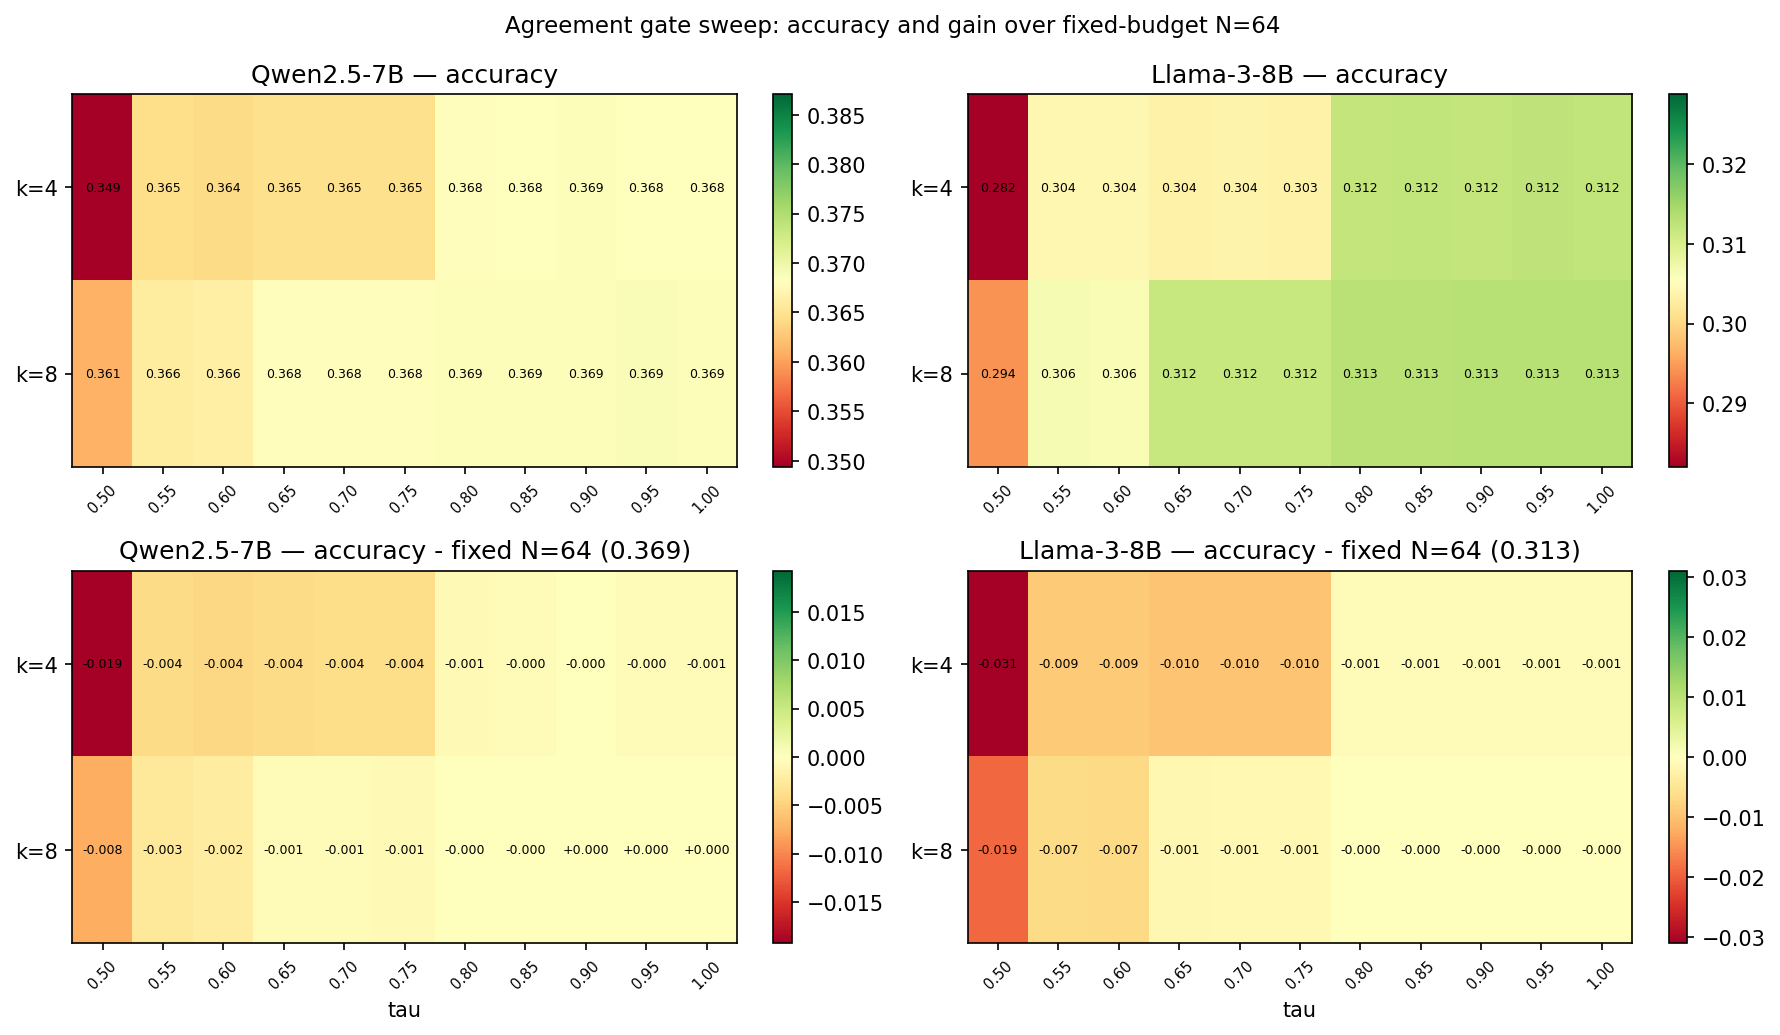
\includegraphics[width=\linewidth]{../outputs/gate_model2/gate_sweep_both.png}
\end{center}
\caption{Agreement-gate accuracy across the $(k, \tau)$ sweep, relative to
fixed-budget at matched compute. No operating point wins.}
\label{fig:sweep}
\end{figure}

\subsection{Why: confidence does not track correctness}

The reason is direct (Table~\ref{tab:calibration}, Figure~\ref{fig:calibration}).
Binning problems by how concentrated the model's answers are, even the
highest-agreement bin is far from reliable: Qwen's plurality is correct 52.5\%
of the time there, and Llama's only 28.6\%, lower than its own low-agreement
bin. Llama's accuracy decreases as agreement rises, an anti-calibration
pattern. High self-consistency is therefore confidently wrong about as often as
confidently right for Qwen, and more often for Llama. A gate that trusts
agreement is reading a signal that does not carry the information it needs.

\begin{figure}[t]
\begin{center}
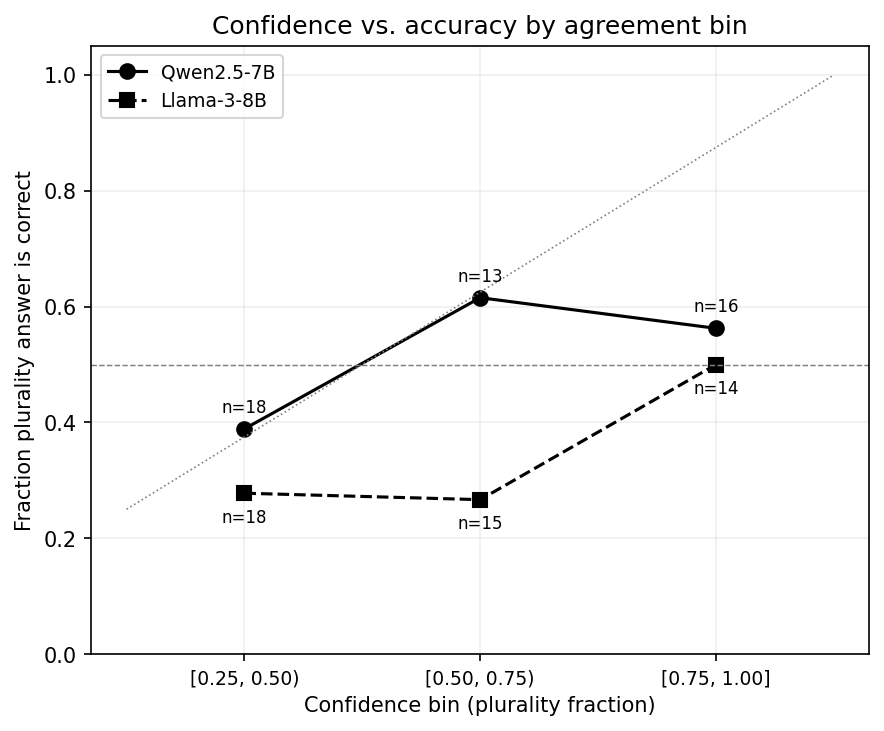
\includegraphics[width=0.6\linewidth]{../outputs/gate_model2/calibration_both.png}
\end{center}
\caption{Fraction of plurality answers correct by agreement bin. Both models
fall far below the calibration diagonal; Llama trends downward.}
\label{fig:calibration}
\end{figure}

\begin{table}[t]
\begin{center}
\begin{tabular}{lcccc}
\toprule
\textbf{Confidence bin} & \textbf{Qwen $n$} & \textbf{Qwen frac correct} & \textbf{Llama $n$} & \textbf{Llama frac correct} \\
\midrule
{[}0.25, 0.50) & 56 & 33.9\% & 79 & 30.4\% \\
{[}0.50, 0.75) & 83 & 27.7\% & 84 & 33.3\% \\
{[}0.75, 1.00] & 59 & 52.5\% & 35 & 28.6\% \\
\bottomrule
\end{tabular}
\end{center}
\caption{Calibration by agreement bin (pooled 198). Confidence is the
plurality fraction over all samples.}
\label{tab:calibration}
\end{table}

\section{Discussion}

\textbf{Why backfire occurs.} On hard problems the model's sampling
distribution concentrates on a wrong answer, so voting locks in the error.
Backfire is not a sampling artifact; it reflects the per-problem answer
distribution. GPQA distractors are designed to be
plausible~\citep{rein2023gpqa}, which amplifies the effect.

\textbf{Why the gates fail.} Both gates read confidence (agreement, or low
entropy), but confidence on these problems does not indicate correctness, and
for the weaker model is inversely related to it. The calibration data make
this concrete.

\textbf{Positioning.} Prior work established that self-consistency helps on
benchmarks where models have higher baseline
accuracy~\citep{wang2023self}; we show it hurts the majority of problems on a
hard one. Repeated-sampling analyses study coverage under an oracle
metric~\citep{brown2024large}; we instead decompose the gap between realizable
majority vote and the oracle. Adaptive-consistency early
stopping~\citep{aggarwal2023adaptive} is essentially our agreement gate,
validated on easier datasets where backfire is rare; our negative result shows
agreement stability is insufficient on hard problems. The external-signal
direction this motivates, trained verifiers and process reward
models~\citep{cobbe2021training, lightman2023verify}, is the natural way to
reach the oracle headroom, which our two verifier-free gates cannot.

\textbf{Implications.} On hard inputs, do not assume self-consistency is safe,
and do not expect agreement or token entropy to tell you when it is; we tested
both and both fail. Recovering the headroom likely requires a signal external
to the model's own samples.

\section{Limitations}

\textbf{Llama is near chance.} Llama-3-8B's single-sample accuracy on full
GPQA Diamond is 0.273, just above the 0.25 random baseline, so its backfire
is less surprising. Qwen (0.342, clearly above chance) is the stronger
demonstration; Llama corroborates the direction.

\textbf{One benchmark.} All results are on GPQA Diamond, graduate-level
science. Other domains and easier difficulty regimes may differ.

\textbf{Two small, non-reasoning models.} Reasoning-native models require
different infrastructure. We attempted a preliminary evaluation of a
reasoning-native model with hidden chain-of-thought and found that a
substantial fraction of samples exhausted the output token budget on hidden
reasoning before producing a visible answer. This truncation made
majority-vote accuracy incomparable to our non-reasoning models. A proper
evaluation of reasoning-native architectures therefore requires larger
inference budgets and explicit handling of hidden CoT output length, and is
left to future work. Whether backfire shrinks or persists for such models
remains the central open question.

\textbf{Subset representativeness.} The original 47-problem subset was easier
than the full benchmark (Qwen $N=1$ accuracy 0.418 vs 0.342 pooled), which is
why we report on all 198.

\textbf{Oracle and ratio.} The oracle is an upper bound, not deployable, and
the fraction-of-oracle-captured ratio is noisy (small denominator), so we lead
gate claims with absolute accuracy.

\textbf{Known mechanism.} Confidence failing to track correctness is an
instance of documented overconfidence~\citep{guo2017calibration,
kadavath2022language}; our contribution is the pre-registered, replicated,
self-consistency-specific quantification and the failure of two cheap gates,
not the existence of miscalibration.

\section{Conclusion}

On hard reasoning problems, self-consistency backfires on the majority of
problems, pre-registered and confirmed across two model families on the full
GPQA Diamond benchmark. The accuracy this leaves on the table is real but
unreachable with a verifier-free agreement or entropy gate, because confidence
does not track correctness. Whether reasoning-native models escape this is the
key open question.

\bibliography{references}
\bibliographystyle{colm2026_conference}

\end{document}
